% Options for packages loaded elsewhere
\PassOptionsToPackage{unicode}{hyperref}
\PassOptionsToPackage{hyphens}{url}
%
\documentclass[
  10pt,
]{article}
\usepackage{amsmath,amssymb}
\usepackage{iftex}
\ifPDFTeX
  \usepackage[T1]{fontenc}
  \usepackage[utf8]{inputenc}
  \usepackage{textcomp} % provide euro and other symbols
\else % if luatex or xetex
  \usepackage{unicode-math} % this also loads fontspec
  \defaultfontfeatures{Scale=MatchLowercase}
  \defaultfontfeatures[\rmfamily]{Ligatures=TeX,Scale=1}
\fi
\usepackage{lmodern}
\ifPDFTeX\else
  % xetex/luatex font selection
\fi
% Use upquote if available, for straight quotes in verbatim environments
\IfFileExists{upquote.sty}{\usepackage{upquote}}{}
\IfFileExists{microtype.sty}{% use microtype if available
  \usepackage[]{microtype}
  \UseMicrotypeSet[protrusion]{basicmath} % disable protrusion for tt fonts
}{}
\makeatletter
\@ifundefined{KOMAClassName}{% if non-KOMA class
  \IfFileExists{parskip.sty}{%
    \usepackage{parskip}
  }{% else
    \setlength{\parindent}{0pt}
    \setlength{\parskip}{6pt plus 2pt minus 1pt}}
}{% if KOMA class
  \KOMAoptions{parskip=half}}
\makeatother
\usepackage{xcolor}
\usepackage[margin=.8in]{geometry}
\usepackage{graphicx}
\makeatletter
\def\maxwidth{\ifdim\Gin@nat@width>\linewidth\linewidth\else\Gin@nat@width\fi}
\def\maxheight{\ifdim\Gin@nat@height>\textheight\textheight\else\Gin@nat@height\fi}
\makeatother
% Scale images if necessary, so that they will not overflow the page
% margins by default, and it is still possible to overwrite the defaults
% using explicit options in \includegraphics[width, height, ...]{}
\setkeys{Gin}{width=\maxwidth,height=\maxheight,keepaspectratio}
% Set default figure placement to htbp
\makeatletter
\def\fps@figure{htbp}
\makeatother
\setlength{\emergencystretch}{3em} % prevent overfull lines
\providecommand{\tightlist}{%
  \setlength{\itemsep}{0pt}\setlength{\parskip}{0pt}}
\setcounter{secnumdepth}{5}
\usepackage{graphicx,longtable,booktabs,here,threeparttable}
\usepackage{float}
\usepackage{pdfpages}
\usepackage{setspace}\singlespacing
\floatplacement{figure}{H}
\floatplacement{table}{H}
\usepackage{xcolor,lipsum}
\usepackage{caption}
\captionsetup[table]{labelfont=bf}
\usepackage[round]{natbib}
\usepackage{pdflscape}
\usepackage{lscape}
\usepackage{etoolbox}
\newcommand{\blandscape}{\begin{landscape}}
\newcommand{\elandscape}{\end{landscape}}
\usepackage{array} \newcolumntype{L}[1]{>{\raggedright\let\newline\\\arraybackslash\hspace{0pt}}m{#1}} \newcolumntype{C}[1]{>{\centering\let\newline\\\arraybackslash\hspace{0pt}}m{#1}} \newcolumntype{R}[1]{>{\raggedleft\let\newline\\\arraybackslash\hspace{0pt}}m{#1}}
\ifLuaTeX
  \usepackage{selnolig}  % disable illegal ligatures
\fi
\usepackage[]{natbib}
\bibliographystyle{plainnat}
\usepackage{bookmark}
\IfFileExists{xurl.sty}{\usepackage{xurl}}{} % add URL line breaks if available
\urlstyle{same}
\hypersetup{
  pdftitle={Supplementary Content},
  hidelinks,
  pdfcreator={LaTeX via pandoc}}

\title{Supplementary Content}
\usepackage{etoolbox}
\makeatletter
\providecommand{\subtitle}[1]{% add subtitle to \maketitle
  \apptocmd{\@title}{\par {\large #1 \par}}{}{}
}
\makeatother
\subtitle{Is There a Competitive Advantage to Using Multivariate
Statistical or Machine Learning Methods Over the Bross Formula in the
hdPS Framework for Bias and Variance Estimation?}
\author{}
\date{\vspace{-2.5em}}

\begin{document}
\maketitle

\appendix
\counterwithin{figure}{section}
\counterwithin{table}{section}

\edef\tablename{\appendixname~\tablename}
\edef\figurename{\appendixname~\figurename}

\section{Variables Used for Plasmode Simulation Data
Generation}\label{variables-used-for-plasmode-simulation-data-generation}

\begin{enumerate}
\def\labelenumi{\arabic{enumi}.}
\tightlist
\item
  Original demographic variables (8)
\end{enumerate}

\begin{itemize}
\tightlist
\item
  age,
\item
  sex,
\item
  education,
\item
  race,
\item
  marital status,
\item
  income,
\item
  country where born,
\item
  survey cycle
\end{itemize}

\begin{enumerate}
\def\labelenumi{\arabic{enumi}.}
\setcounter{enumi}{1}
\tightlist
\item
  Original behaviour variables (5)
\end{enumerate}

\begin{itemize}
\tightlist
\item
  smoking,
\item
  diet,
\item
  high cholesterol,
\item
  physical activity,
\item
  sleep
\end{itemize}

\begin{enumerate}
\def\labelenumi{\arabic{enumi}.}
\setcounter{enumi}{2}
\tightlist
\item
  Original health history / access variables (2)
\end{enumerate}

\begin{itemize}
\tightlist
\item
  diabetes family history,
\item
  medical access
\end{itemize}

\begin{enumerate}
\def\labelenumi{\arabic{enumi}.}
\setcounter{enumi}{3}
\tightlist
\item
  Transformed lab variables (6) (complex forms) based on original lab
  variables: uric acid, protein, bilirubin, phosphorus, sodium,
  potassium, globulin, calcium, systolic blood pressure, diastolic blood
  pressure.
\end{enumerate}

\begin{itemize}
\tightlist
\item
  Tranfored.var.1 = log(globulin)
\item
  Tranfored.var.2 = protein*calcium
\item
  Tranfored.var.3 = diastolicBP/systolicBP)\^{}2
\item
  Tranfored.var.4 = sqrt(uric acid+bilirubin)/2
\item
  Tranfored.var.5 = phosphorus\^{}2/(sodium*potassium)
\item
  Tranfored.var.6 = log(systolicBP+10)
\end{itemize}

\begin{enumerate}
\def\labelenumi{\arabic{enumi}.}
\setcounter{enumi}{4}
\tightlist
\item
  Count based prescription codes (1) (proxies of comorbidity)
\end{enumerate}

Simple count (1 variable) = sum of selected ICD-10 CM codes (converted
to recurrence covariates) who had less than 0.8 or greater than 1.2
compared to the outcome = \(\sum_{s=1}^{94} R_s\)

\section{True Outcome Model for Plasmode Simulation Data
Generation}\label{true-outcome-model-for-plasmode-simulation-data-generation}

Diabetes (outcome) = Obese (exposure) + demographic/behaviour/health
history variables + transformed lab variables + simple count with
selected ICD-10 codes

\section{Standard Error comparison}\label{standard-error-comparison}

\begin{figure}

{\centering 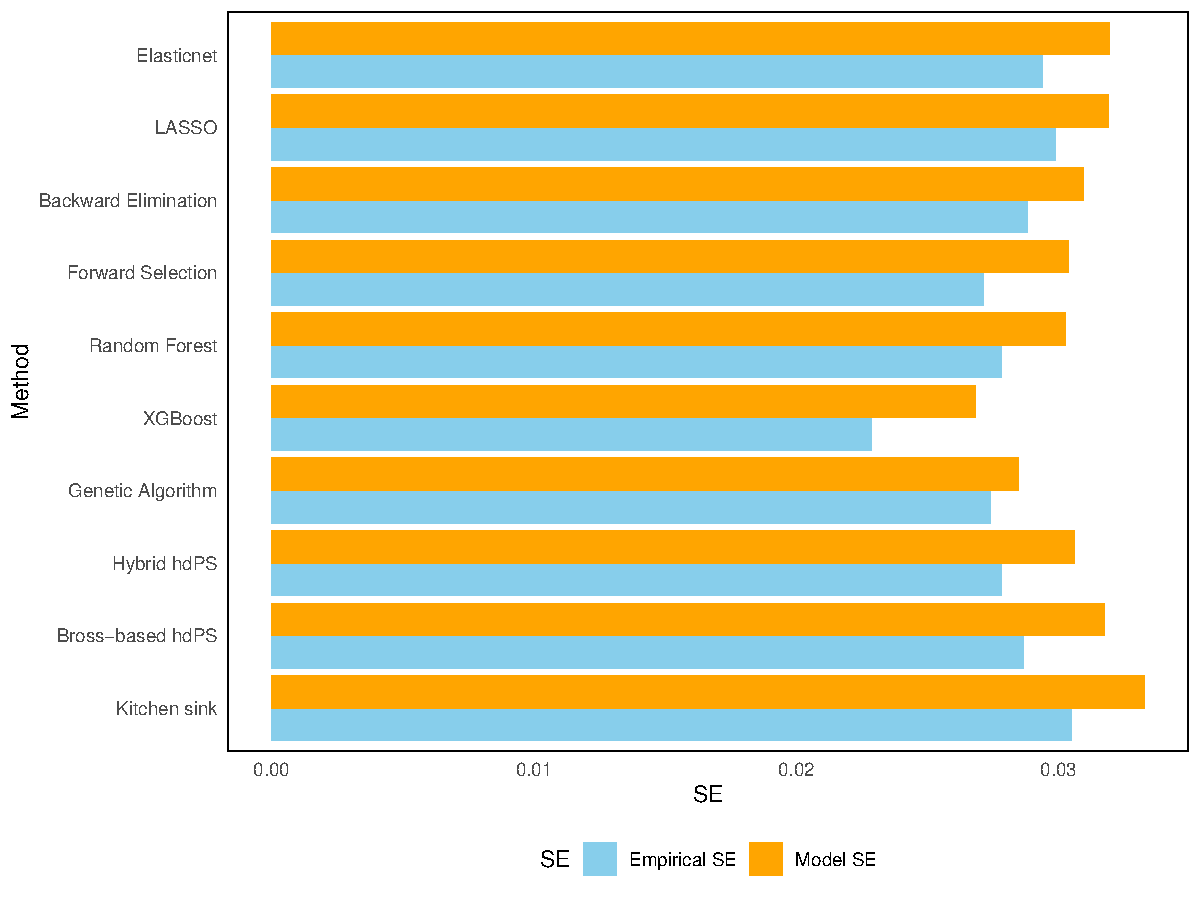
\includegraphics[width=1\linewidth]{se_comparison_plot} 

}

\caption{Standard Error Comparison for Different Methods (Overall) when outcome and exposure are frequent.}\label{fig:unnamed-chunk-1}
\end{figure}

\begin{figure}

{\centering 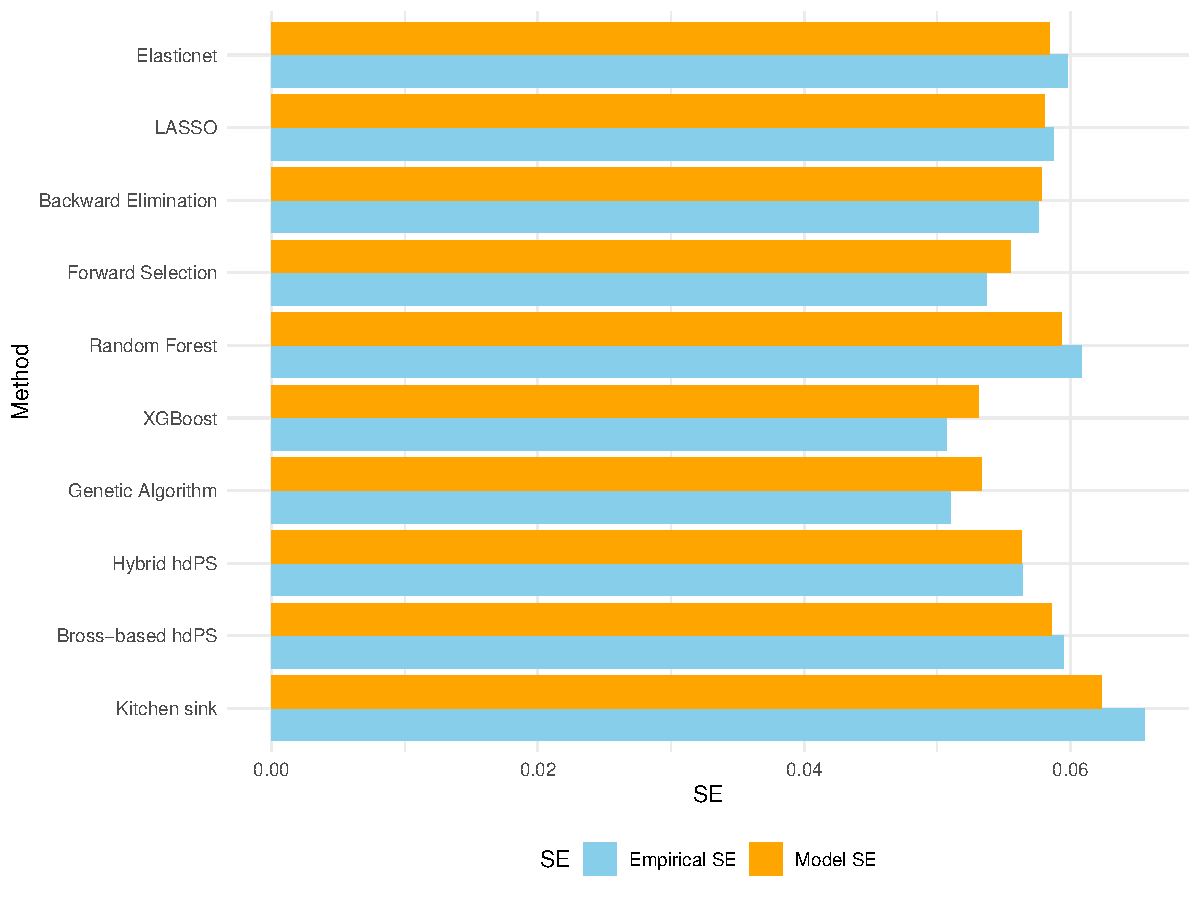
\includegraphics[width=1\linewidth]{se_comparison_plotER} 

}

\caption{Standard Error Comparison for Different Methods (Overall) when outcome is frequent but exposure is rare.}\label{fig:unnamed-chunk-2}
\end{figure}

\begin{figure}

{\centering 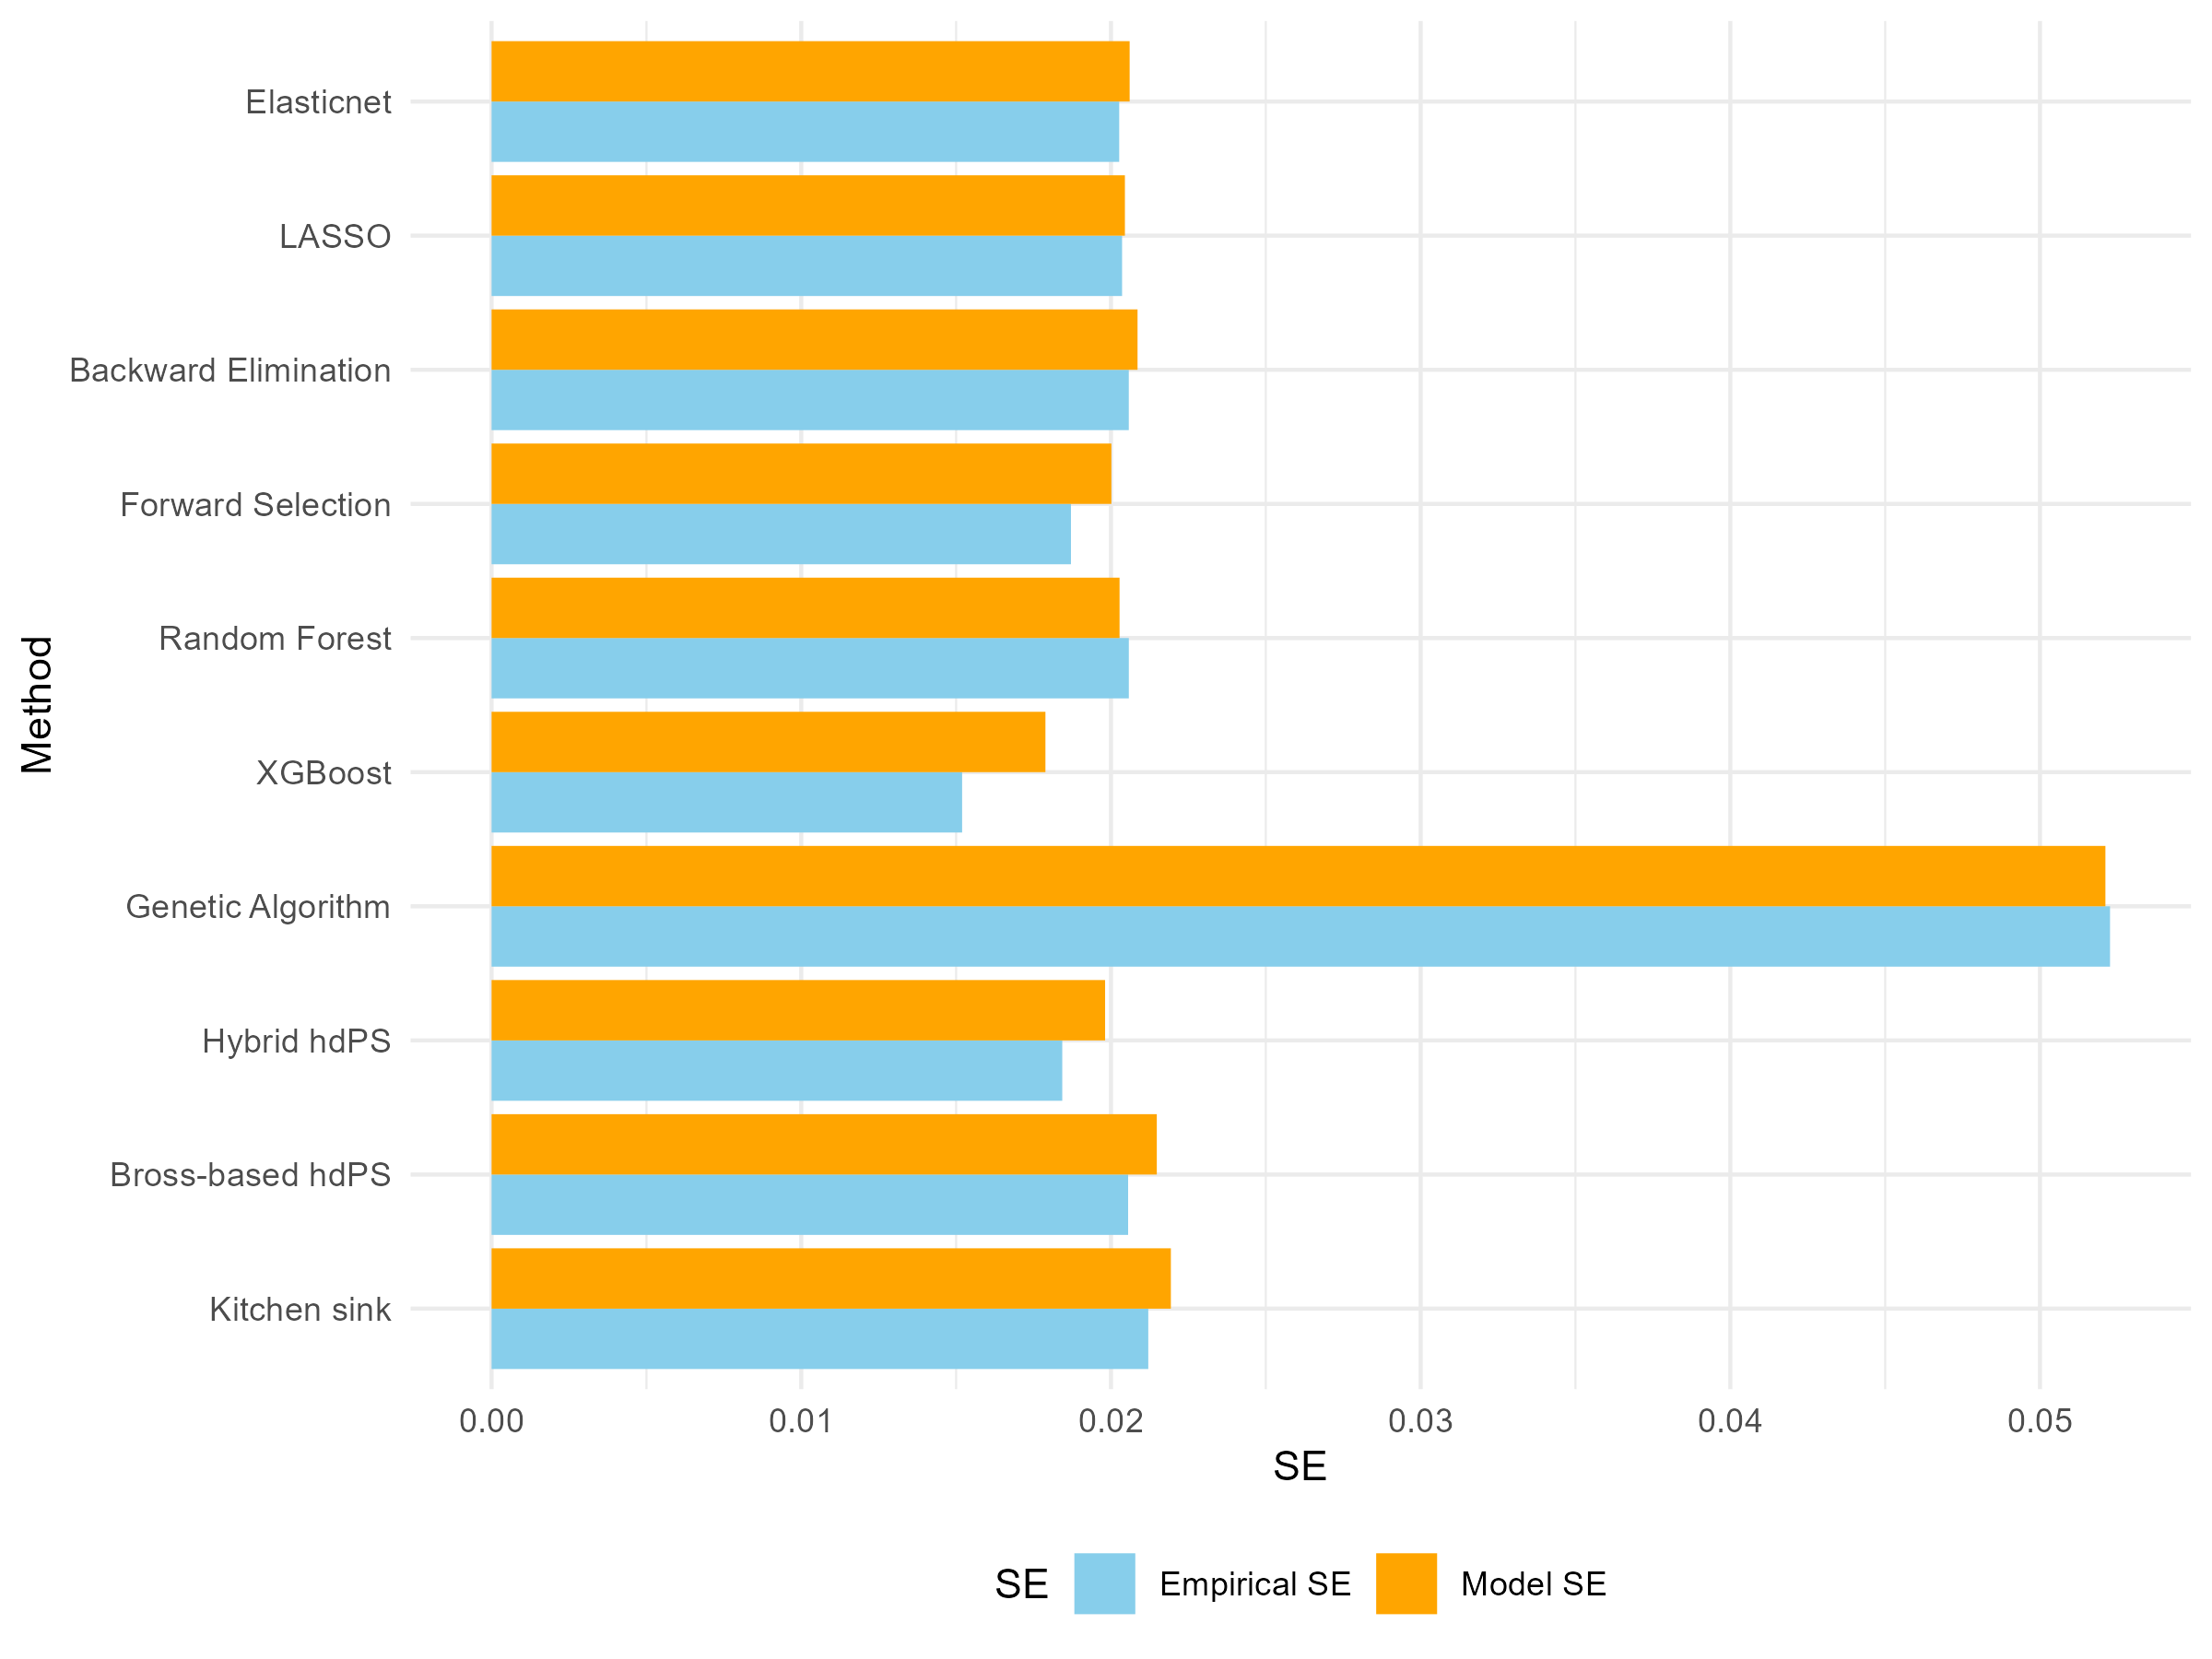
\includegraphics[width=1\linewidth]{se_comparison_plotOR} 

}

\caption{Standard Error Comparison for Different Methods (Overall) when outcome is rare but exposure is frequent}\label{fig:unnamed-chunk-3}
\end{figure}

  \bibliography{mergedbibliography.bib}

\end{document}
